\documentclass[a4paper,11pt]{book}
%
% The current document is based on a document by Marten Wortel
% who is greatly acknowledged for making his document available
%
\usepackage{amsmath,amsthm,amsfonts,mathrsfs,anysize,fancyhdr,epsfig,svg}

%\usepackage[section]{placeins}
\usepackage{tikz}

\newcommand{\bb}{\mathbb}
\newcommand{\mb}{\mathbf} \newcommand{\mc}{\mathcal}
\newcommand{\pred}{\mathrm{Pred}}
\newcommand{\ov}{\overline}

\newtheorem{theorem}{Theorem}
\newtheorem{proposition}{Proposition}
\newtheorem{property}{Property}
\newtheorem{lemma}{Lemma}
\newtheorem*{corollary}{Corollary}

\theoremstyle{definition}
\newtheorem{definition}{Definition}
\newtheorem{conjecture}{Conjecture}
\newtheorem*{example}{Example}
\newtheorem{algorithm}{Algorithm}

\graphicspath{ {plots_all/} }

\usetikzlibrary{positioning}


\begin{document}

\begin{titlepage}

\thispagestyle{empty}

{\hspace{10cm}
\begin{minipage}{5cm}
  
\includegraphics{tudelft.eps}
\end{minipage}}

\begin{center}

\vspace{1.0cm}

\large
\textbf{\large{Delft University of Technology}} \\
\textbf{\large{Faculty of Electrical Engineering, Mathematics and Computer Science}} \\
\textbf{\large{Delft Institute of Applied Mathematics}}

\vspace{2.0cm}

\framebox[16cm]{\raisebox{0cm}[1.5cm][1.5cm]
 {\textbf{
   \begin{minipage}{13cm}\Large
   \begin{center}
       Sybil-resistant trust mechanisms in distributed systems
   \end{center}
   \end{minipage}}}}

\vspace{2.0cm}

\large A thesis submitted to the\\
Delft Institute of Applied Mathematics\\
in partial fulfillment of the requirements

\vspace{1.0cm}

for the degree\\

\vspace{1.0cm}

\textbf{\large{MASTER OF SCIENCE} \\
in \\
\large{APPLIED MATHEMATICS} \\
\vspace{1cm}
by}

\vspace{1cm}

\textbf{PIM OTTE}\\

\vspace*{\stretch{2}}

\textbf{Delft, the Netherlands \\
August 2016} \\

\vspace{1cm}

Copyright \copyright{} 2016 by Pim Otte. All rights reserved.
\end{center}

\end{titlepage}

\newpage

\thispagestyle{empty}

\quad

\newpage

\thispagestyle{empty}

\hspace{10cm}
\begin{minipage}{5cm}
  
\includegraphics{tudelft.eps}
\end{minipage}

\begin{center}
\vspace*{\stretch{1}}

\textbf{\large{MSc THESIS APPLIED MATHEMATICS}}

\vspace{1.5cm}

\textbf{``Considering temporal factors in distributed trust''}

\vspace{1.5cm}

PIM OTTE\\

\vspace{1.5cm}

\textbf{\large{Delft University of Technology}}

\vspace{\stretch{5}}

\end{center}

\begin{center}
\begin{tabular}{ll}
\large{\bf{Daily supervisors}} & \large{\bf{Responsible professor}} \\
$\;$ & \\
\large{Dr.~D.~C.~Gijswijt}  & \large{Prof.\ dr.~ir.~K.~Aardal} \\
$\;$ & \\
\large{Dr.~J.~Pouwelse} & \phantom{niets} \\
\phantom{niets} & \phantom{niets} \\
$\;$ & \\
\phantom{niets} & \phantom{niets} \\
$\;$ & \\
\phantom{niets} & \phantom{niets} \\
$\;$ & \\
\phantom{niets} & \phantom{niets} \\
$\;$ & \\
\phantom{niets} & \phantom{niets} \\
$\;$ & \\
\large{August 2016} & \large{Delft, the Netherlands}
\end{tabular}
\end{center}
\newpage

\thispagestyle{empty}

\quad

\newpage

%TODO make figures black-white compatible 
\chapter*{\centering \begin{normalsize}Abstract\end{normalsize}}

In this thesis, the problem of estimating trust in a distributed network is considered.

\clearpage
\tableofcontents
\pagenumbering{arabic}
\chapter{Introduction}
    
Nowadays, the internet is an absolutely critical piece of infrastructure. According
to the International Telecommunication Union, 47\% of the world population uses the internet.
In the developed world, 81\% of the inhabitants uses the internet~\cite{itu2016facts}.
The internet is used for important communication and banking, education, but also for entertainment and
leisure. Internet access has not quite
made it to being a basic human right. However, the United Nations Special Rapporteur
on the promotion and protection of the right to freedom of opinion and expression, wrote
the following on the matter in a report~\cite{larue2011report}:

\begin{quote}
    ``\textit{there should be as little restriction as possible  to  the  flow  of  information  via  the  Internet,
    except  in  few,  exceptional,  and  limited  circumstances  prescribed  by  international  human  rights  law.}'' 
    
    -Frank La Rue  
\end{quote}

This leaves little doubt that the availibility of the internet is protected by Article 19 of the
the Universal Declaration of Human Rights ``Freedom of Opinion and Information''.

A more controversial issue has been going on for longer than it is known to the general public.
In 2013, Edward Snowden disclosed the first of several pieces of information that
have shown digital communication, the internet included, is subject to extensive surveillance.
Also known as the ``Snowden Revelations'', the information released consists of a series
of documents and accompanying articles. The documents originate from several intelligence 
agencies and detail the scale and methods with which these agencies perform digital
surveillance. 
About this, David Lyon writes the following~\cite{lyon2014surveillance}

\begin{quote}
    ``\textit{Given the reliance on western liberal legal traditions
    it is hardly surprising that public debate generally 
    commences around the question of} privacy. 
    \textit{Understood as a human right, it underlies aspects of democratic polity,
    such as freedom of expression. 
    Often understood in the post-Snowden era as relating to 
    control of communications about oneself, 
    it is clearly a threatened value if not – according to some – a forlorn hope.}

    -David Lyon
\end{quote}

Hence, if we value the human rights to freedom of expression and privacy, then an internet
with entities performing unbounded surveillance is not desirable. 

On the one hand, even back in 2001 there was a a growing consensus that the internet poses
a threat to the existance of authoritarian regimes~\cite{kalathil2001internet}. 
On the other hand, regimes like China~\cite{endeshaw2004internet} and Iran~\cite{kimppa2010emancipatory}
try their very best to censor content. 

The solutions to ensuring availibility of the internet and its services
appears to to have one thing in common. All systems aiming to do so leverage the concept of
a \emph{distributed system}. Distributed systems are networks of computers that all perform part
of a common task. The advantage of distributed systems is that, if well designed, they are
extremely hard to take down. The disadvantage of a distributed systems is that there will
be difficulties in the distribution, in particular if the the system is actually physically
distributed. 

A prime example of using a distributed system to increase availibility is the 
bittorrent protocol~\cite{cohen2008bittorrent}. This protocol enables something called peer-to-peer filesharing.
In this paradigm, many computers are in possesion of (part of) a file. Computers
which do not possess the enitre file can request little pieces of it from other
computers (also known as peers). This protocol ensures the availibility of this
file. If any peer stops functioning for any reason whatsoever, the rest of
the network can continue to exist as is, as long as all active peers have the
entire file amongst themselves. 

An example of a distributed system that ensure both availibility and privacy is
Tor~\cite{dingledine2004tor}. Tor is a so-called onion routing protocol. 
The concept of onion routing is as follows. One obtains a list of peers in the
network, at least one of which needs to be available as ``exit node''. If one
then wants to communicate with the internet, any request that would normally
be sent directly is instead routed through two or more of these peers, the last
of which must be an exit node. This is done by wrapping the request in one
layer per peer. These layers constitute the onion. The way this is done is such
that each peer in the network knows the previous and next link in this chain,
but no one except the originator knows the entirety. The exit node is the last
hop, and they will send this on to the recipient on the internet. Hence, they
know everything that is not encrypted about this request and response, which includes at
least the recipient. 
The aim of using an onion protocol is to hide the identity of the browsing party. Indeed,
their identity can only be revealed if too many of the peers in the chain are controlled
by the same party. This protocol can be applied to any sort of web traffic, including
bittorrent traffic. 

The techniques of bittorrent and Tor have both been incorporated into another piece
of software: Tribler. Since both of these techniques are quintessentially distributed,
naturally Tribler itself works as a distributed system. This piece of software unifies
several key pieces of technology to provide anonymous bittorrent to its users. In addition,
it provides a distributed search engine for torrent files and a built-in media player in
order to stream a torrent. 

While this piece of software may seem to be the ultimate tool of an internet pirate, 
allow us to consider it in the light of the human rights mentioned above. Due to its
distributed nature, Tribler is much less susceptible to traditional filtering and
censoring techniques. In particular, unless all connectivity to a peer is severed,
there is very little an authoritarian regime can do once a user gets their hands
on Tribler. This enables information to freely flow from peer-to-peer and hence 
enables Frank La Rues vision of as little restriction as possible. 
Furthermore, the other side of the human rights equation considers the human
right to privacy. That Tribler offers this is not a point of discussion. What might
be considered is the question of whether Tribler offers too much privacy. Does it
prevent law enforcement from doing their job? Does Tribler impact the war on terror?
One might argue that Tribler does in fact offer too strong of a protection.
However, the legal measures law enforcement can take, like a digital
wiretap specific to a person or computer, are not prevented by Tribler. What is
prevented is the style of mass surveillance uncovered by the Snowden revelations. 

Distributed systems seem to be all sunshine and no rain. Protecting human rights 
and ensuring availibility of services. However, the decentralization does pose certain 
problems. One problem in particular is resource management. A decentralized system
like Tribler has many of the same properties as the climate change problem. Most of the
world is aware climate is changing and that a change in their behavior would help to
mitigate this problem. In fact, if the world as a whole does not alter their behavior,
there might be catastrophic consequences. However, the impact a single person or household
has is extraordinarily small. So small, that most people reason that their behavior
does not impact the world, so they will just continue living as they always have. 
This problem is known as the Tragedy of the Commons. Everyone would win if everyone
participated, but one person can not make the difference. 
This concept has been study at length in the past decades, we refer to
Hardin~\cite{hardin2009tragedy} for a view of this problem in broader society.
In Tribler, this concept exists in the following form: Everyone would like to use 
the network to download data. However, in order to do so, there needs to be at least
one agent to relay this data, and then another one to request it from the internet.
This means that if enough agents fulfill these functions out of their free will,
and everyone does a little bit, the load will be spread and the network will
fuction. However, it is much more enticing to not contribute and only consume.

Traditionally, in bittorrent networks, this problem has been solved for public torrents
by simply relying on altruistic agents, who contribute based on nothing more than
their good will. There also exists the concept of a private community, in which a central
entity records how much data is downloaded and uploaded by each agent. This central
entity then does ``ratio enforcement'' and excludes members that drop below a certain
contribution ratio. Tribler has so far mostly relied on the altruists. 
Recently, a movement has started to bring some sort of trust system to Tribler. In particular,
if an agent considers another one to be trustworthy, in the sense that they have contributed
a lot to the network, the former would give the latter priority in requests for resources.

The problem here is that since the system itself needs to maintain anonimity, the task of
finding out if an agent is contributing suddenly becomes a lot harder. In particular, 
it becomes very hard to determine whether an agent is real, and has had interactions with
others, if one can not have an interaction with this agent themselves. An agent could simply
exist by claim of another, including fictional interactions with the real agent. Any trust system
should therefore be able to deal with such attacks. The theoretical resistance to attacks,
and the performance in practice are the subjects of this thesis.



\chapter{Research questions}

As argued in the introduction, distributed systems can have advantages over traditional centralized
systems. However, distributing a system comes with several challenges, in particular that
the agents in this system will need to contribute in order for the system to
function. This can easily lead to a tragedy of the commons, where everyone is slacking,
but the result would be better if everyone pitched in a small amount of effort.

The focus of this thesis is the following research question:

\begin{center}
    Can agents in a distributed network use confirmed information about
    interations and their order to judge the reputation of other agents
    in a fair and efficient way?
\end{center}

Before anything else, we need to specify what ``judge the reputation'' means.
An agent will judge the reputation of others by assigning each of them a score.
If one agent is assigned a higher score than another, the former is judged to be more
reputable.  These scores could then be used to determine priority in distributing resources.

Throughout this thesis we will consider Tribler as an application area and experimental
evaluation will be done using Tribler. 
In this context, a system that assigns a score
to agents given information about their interactions has been dubbed an 
``accounting mechanism'' by Seuken~and~Parkes~\cite{seuken2010accounting}. This
work will adhere to this terminology.

To restrict the scope of this research, only accounting mechanisms are considered as a method
of using the information about the order of interactions. This reduces the main research question
to the following:

\begin{center}
    Does information about the order of interactions allow the design of an accounting mechanism
    that satisfies the following three properties?
\end{center}

\begin{itemize}
    \item The accounting mechanism is fair. 
    \item The accounting mechanism is manipulation-resistant.
    \item The accounting mechanism is efficiently computable.
\end{itemize}

These properties are far from well-defined in this context, so let us consider each of them.

\section{Fairness}

The meaning of fairness as in the above property is that the score assigned to an agent
accurately reflects their contribution. The problem with this is that the target might
vary for different application domains. For example, in the context of a social
network where interactions are friendships, interactions are positive for both sides.
In a system like Tribler, interactions will be positive for at least one side, but
might have a negative impact on the reputation. In a distributed system like Bitcoin,
we might interpret the amount of money an agent posesses as a score assigned. In
this case, the transfer of money is the interaction, and it will be positive for one
agent and negative for the other.

For purposes of this thesis we will zoom in on fairness in the context of Tribler.
This notion would hold up for other distributed systems in case that each node
can contribute or consume resources, where contributing is positive, consuming
is negative, and contributing and consuming the same amount is explicitly seen as postive.
Generally, in bittorrent networks, the ratio between upload and download is seen
as a fair measure of contribution. However, since in Tribler, relaying data for onion
routing is a service that the network provides, uploading and downloading the same
amount is seen as a postive thing. This is not reflected in the ratio, which
means that we cannot take it as an accurate representation of a fair accounting mechanism.

To at least get some notion of what constitutes fair, let us consider an agent that
engages in a new interaction. Then the following would be an indication of a fair mechanism:

\begin{itemize}
    \item If the agent consumes more resources than they contribute, their score goes down.
    \item If the agent consumes less resources than they contribute and less than they have
        done historically, their score goes up.
     \item If the agent consumes less resources than they contribute, but more than they have
        done historically, their score might not change.
\end{itemize}

\section{Resistance to manipulation}

While fairness says something about the score in relation to the actions within
the system, resistance to manipulation concerns actions that are not ``normal''
in the system. In particular, lying of any sort, creating extra or new identities
and any other actions than participating in the network should not lead to an
increase in score.

\section{Efficiency of computation}

As well known, the efficiency of algorithms can be compared with big-$O$ notation.
It might vary per application domain if an accounting mechanism with a certain
theorethical worst-case performance is useable. It might be that some
theoretically slow mechanisms turn out to be fast in practice, or that the
instance sizes are small enough to allow a higher-order algorithm. Hence,
in addition to big-$O$ notation, the efficiency will be studied in practice.



\chapter{Base Model of Interaction Information}

In order to exploit information about interactions, this information will need to be
available in the first place. In order to allow general applicability of the
techniques, first the general model is considered, which is then shown to be
relevant in the particular case of the software known as ``Tribler''.


\section{Base model}

In order to incorporate temporal information in sybil defense mechanisms,
there will be some assumptions needed about the information which is available.
Hence, applications which fit the following model will be explored.

\begin{definition}[Ordered interaction model]
    An \emph{ordered interaction model} $M$ consists of two sets:  
    
    \begin{itemize}
        \item $P$, a finite set of agents
        \item $I$, a finite partially ordered set of interactions
    \end{itemize}

    Agents represent entities that can interact with each other.
    An interaction consists of two different agents, one or both performing
    work for each other. 
    
    An interaction is defined by two pairs of properties:
    \begin{enumerate}
        \item $p, q \in P$, two agents involved in the interaction.
        \item $w_p, w_q \in \bb{R}_{\geq0}$, representing amount of work done by $p$, respectively $q$.
    \end{enumerate}

    Furthermore, for each $p \in P$, the partial order on $I$ must induce a total order on:
    \begin{equation*}
        I_p = \{i \in I : p \mbox{ is an agent in } i\}
    \end{equation*}
\end{definition}

This model is designed such that the Tribler use case can be mapped to it. However, this model is
generic enough that it might be applied in other situations. In particular, any system where
agents interact and perform work for each other, where this work can be quantified in a number,
this model can be applied to. In most cases, the ordering on the interaction will be relatable
to time.

\begin{definition}[Successor of an interaction]
     If $i, j \in I$, $i < j$, and there exists no $i'$ such that $i < i' < j$, then
$j$ is a successor of $i$. This is denoted by $i \preceq j$.
\end{definition}
 
This model induces a graph that resembles traditional interaction graphs, but preserves the knowledge
of the order of interactions.
\begin{definition}[Ordered interaction graph]
    The directed graph $G_M = (V, A)$ is defined as the \emph{ordered interaction graph} derived from an ordered interaction model $M = (P,I)$.
    Its structure is as follows:

    \begin{itemize}
        \item $V := \{ v_{i} : i \in I\}$\\
        \item $A := \{ (v_{i}, v_{j}) : i, j \in I, \mbox{ s.t. } i \preceq j \}$\\
    \end{itemize}

    In contexts where not defined otherwise, the weight of an arc is the amount of the work performed by $p$ in
    interaction $i$. 
\end{definition}


\begin{definition}[Block Graph]
    Let $M = (P, I)$ be an ordered interaction model. The block graph $G^B_{M}$ is defined as follows:

    \begin{itemize}
        \item $V := \{ v_{p, i} : i \in I, p \mbox{ an agent involved in } i \}$\\
        \item $A := \{ (v_{p,i}, v_{q,j} : i, j \in I \mbox{ s.t. } i \preceq j \}$\\
    \end{itemize}

    This graph can be weighted. Let $(v_{p,i}, v_{q, j}) = a \in A$, then:

    \begin{equation*}
        w(a) := \mbox{ The amount of work } q \mbox{ has performed in interaction } i 
    \end{equation*}
\end{definition}


\begin{definition}[Interaction Graph]
    Let $M = (P, I)$ be an ordered interaction model. The interaction graph $G^I_M$ is defined as follows:

    \begin{itemize}
        \item $V := \{ v_p : p \in P \}$\\
        \item $A := \{ (v_p, v_q) : p, q \in P \mbox{ s.t. } \exists i \in I \mbox{ involving } p \mbox{ and } q$ \\
    \end{itemize}

    This graph has weights. Let $(v_{p}, v_q) = a \in A$, then:

    \begin{equation*}
        w(a) := \mbox{ The total amount of work } p \mbox{ has performed for } q
    \end{equation*}
\end{definition}

In order to shed more light on these definitions, let us consider an example. This example involves
3 agents: $P, Q, R$. The interactions are as follows:

\begin{table}[h]
    \centering
    \begin{tabular}{c|c|c|c|c|c|c}
        Interaction Id & Agent 1 & Seq 1 & Contribution 1 & Agent 2 & Seq 2 & Contribution 2 \\\hline
        P1Q1           & P       & 1                 & 5MB            & Q       & 1                 & 3MB            \\
        P2R1           & P       & 2                 & 7MB            & R       & 1                 & 1MB            \\
        Q2R2           & Q       & 2                 & 3MB            & R       & 2                 & 8MB            \\
        P3R3           & P       & 3                 & 2MB            & R       & 3                 & 3MB            \\
    \end{tabular}
    \caption{Set of interactions for examples}
    \label{tab:interactions}
\end{table}

In Table~\ref{tab:interactions}, the attributes of the interactions are specified. For each interactions the
agents involved are listed, along with their respective contributions, the amount of data uploaded
to the other. In addition, the sequence number (``Seq'') is listed. Recall that the set of interactions of each agent must
be completely ordered as defined by the partial ordering on the set of interactions. The sequence number is
simply the numbering of this set as prescribed by the ordering. This also gives way to an easy way to uniquely
identify an interaction, namely by concatenating the agents with their sequence numbers. This is listed
as the interaction id. Note that the units of the contributions are in MB. This is a foreshadowing of
the next section, in which we consider the application of this model to Tribler, where the contribution in
interactions consists of transferring data.

\begin{figure}[h]
    \centering
     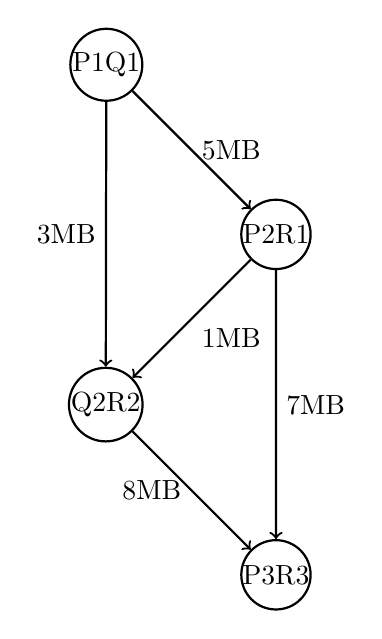
\begin{tikzpicture}[->,thick,scale=0.8,main node/.style={circle, draw, fill=white,
        inner sep=0pt, minimum width=20pt} 
        ]

        \node [main node] (p1q1) {P1Q1} ;
        \node [main node] (p2r1) [below right  = 1.5cm and 1.5cm of p1q1] {P2R1} ;
        \node [main node] (q2r2) [below left = 1.5cm and 1.5cm of p2r1] {Q2R2} ;
        \node [main node] (p3r3) [below right = 1.5cm and 1.5cm of q2r2] {P3R3} ;

        \path[draw, thick]
        (p1q1) edge node [right] {5MB} (p2r1) 
        (p1q1) edge node [left] {3MB} (q2r2) 
        (p2r1) edge node [right] {7MB} (p3r3) 
        (p2r1) edge node [below right] {1MB} (q2r2) 
        (q2r2) edge node [left] {8MB} (p3r3) 
        ;
     \end{tikzpicture}
     \caption{Example of an ordered interaction graph}
     \label{fig:ex_oig}
\end{figure}

Figure~\ref{fig:ex_oig} depicts the ordered interaction graph derived from the data in Table~\ref{tab:interactions}.
Note that some numbers in the graph are not in the graph, as the contributions in an interaction are
weights in the arcs to the successors of that interaction. If that successor does not exist yet, those
contributions have no representant in the graph. The ordered interaction graph functions mainly as a 
structure to consider, as the name says, the order of interactions. It is by definition, the directed
acyclic graph induced by the partial ordering.

\begin{figure}[h]
    \centering
     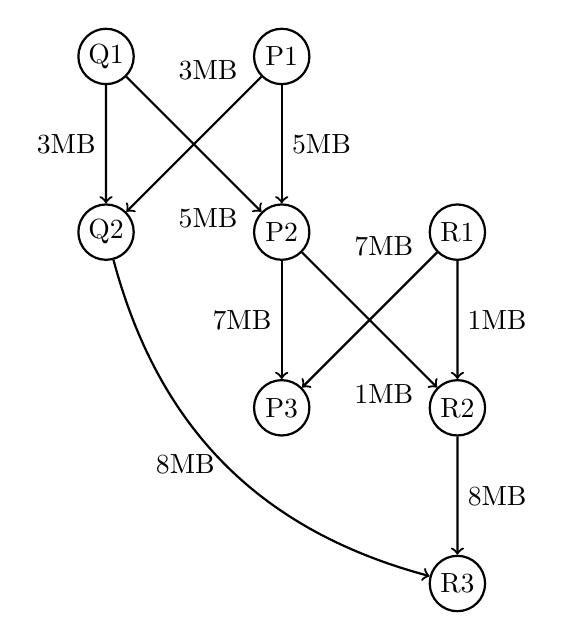
\begin{tikzpicture}[->,thick,scale=0.8,main node/.style={circle, draw, fill=white,
        inner sep=0pt, minimum width=20pt} 
        ]

        \node [main node] (p1) {P1} ;
        \node [main node] (p2) [below = 1.5cm of p1] {P2} ;
        \node [main node] (q1) [left = 1.5cm of p1] {Q1} ;
        \node [main node] (r1) [right = 1.5cm of p2]  {R1} ;
        \node [main node] (r2) [below = 1.5cm of r1] {R2} ;
        \node [main node] (q2) [below = 1.5cm of q1] {Q2} ;
        \node [main node] (r3) [below = 1.5cm of r2] {R3} ;
        \node [main node] (p3) [below = 1.5cm of p2] {P3} ;

        \path[draw, thick]
        (p1) edge node [right] {5MB} (p2)
        (p2) edge node [left] {7MB} (p3)
        (q1) edge node [left] {3MB} (q2)
        (r1) edge node [right] {1MB} (r2)
        (r2) edge node [right] {8MB} (r3)
        (p1) edge node [above left, pos=0.1] {3MB} (q2)
        (q1) edge node [below left, pos=0.9] {5MB} (p2)
        (p2) edge node [below left, pos=0.9] {1MB} (r2)
        (r1) edge node [above left, pos=0.1] {7MB} (p3)
        (q2) edge [bend right] node [left] {8MB} (r3)


        ;
     \end{tikzpicture}
     \caption{Example of a block graph}
     \label{fig:ex_block}
\end{figure}

In Figure~\ref{fig:ex_block} an example of a block graph can be found. This graph has largely the same structure
as the ordered interaction graph, except that each interaction is split into parts belonging to each respective
party. In the case of MultiChain, this representation really shows the chain aspect of this datastructure,
in the sense that each agent has their own sequence of nodes, with additional arcs denoting the interactions.
Again, the lack of representation of the last interactions can be seen. This graph will be used
in Chapter~\ref{chap:temporal_pr} to serve as the basis for Temporal PageRank.


\begin{figure}[h]
    \centering
     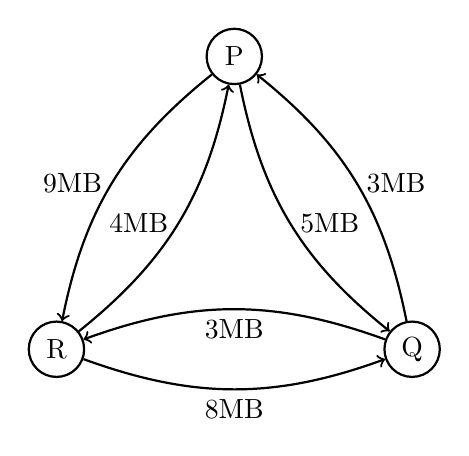
\begin{tikzpicture}[->,thick,scale=0.8,main node/.style={circle, draw, fill=white,
        inner sep=0pt, minimum width=20pt} 
        ]

        \node [main node] (p) {P} ;
        \node [main node] (q) [below right = 3.46cm and 2cm] {Q} ;
        \node [main node] (r) [below left = 3.46cm and 2cm] {R} ;

        \path[draw, thick]
        (p) edge [bend right=20] node [right] {5MB} (q)
        (q) edge [bend right=20] node [right] {3MB} (p)
        (p) edge [bend right=20] node [left] {9MB} (r)
        (r) edge [bend right=20] node [left] {4MB} (p)
        (q) edge [bend right=20] node [below] {3MB} (r)
        (r) edge [bend right=20] node [below] {8MB} (q)
        ;
     \end{tikzpicture}
     \caption{Example of an interaction graph}
     \label{fig:ex_ig}
\end{figure}

Finally, Figure~\ref{fig:ex_ig} shows the interaction graph. Traditionally, this is the graph
that has been used in literature. However, when considering an ordered interaction model, this
graph is the one that might be less obvious at first glance. The structure of the graph
is the block graph with a contraction of all nodes per agent. The weights on the arcs are
the sums of the edges in the block graph, but in the other direction. This graph does
not reflect the notion of time or order in any way. It will be the basis for the
NetFlow mechanism presented in Chapter~\ref{chap:netflow}.



\section{Base model applied to Tribler}

To obtain more insight into the ordered interaction model, consider the following application:

Tribler is an anonymous peer-to-peer file sharing client. In the application of the model,
the set of agents consists of Tribler clients. Each Tribler client is uniquely identifiable,
but a single real world entity could have multiple agents. In Tribler an interaction
consists of two agents uploading data to each other. The amount of work $w_p$ performed
by an agent $p$ is the amount of megabytes uploaded to their peer ($q$), in MB.

In Tribler, these interactions are recorded in a distributed datastructure, called the MultiChain.
Every client saves and signs their interactions, marked with a sequence number. They will then request
a digital signature from their peer, who will mark the interaction with their own sequence number.
These sequence numbers induce a partial ordering, where $i < j$, if and only if there exists
a sequence $(i_0, i_1, \ldots i_n)$, where $i=i_0, j=i_n$ and every pair $(i_k, i_{k+1})$ has
a common agent, for which the sequence number in $i_k$ is lower than in $i_{k+1}$.
This results in a full order on $I_p$, since in that case $(i, j)$ is a valid sequence if
$i$ occurred before $j$ and both involve agent $p$.

The above reasoning shows that the base model as presented is compatible with Tribler as a usecase.
Let us further elaborate on some of the properties of the MultiChain, in order to sketch a better image.
The MultiChain has first been introduced by Norberhuis~\cite{norberhuis2015multichain}. For a detailed
view into this structure, we refer to this work.

There are two main properties of MultiChain that are exploited in the mechanisms this work builds upon it.
Firstly, there is the fact that a record of an interaction can only exist if both parties agree that it
is accurate. Secondly, the MultiChain is built such that there is eventual detection of lying. In particular,
if an agent spreads differing interations to different agents, this will be detected. In terms of the model,
if an agent spreads interactions such that his set of interactions has no total order, the network will
be able to detect and prove this. 

There are also properties of the MultiChain that are less desirable. In particular, with no implementation
will all agents get all the interactions at the same time. In fact, in some possible implementations, 
agents will not even get a full view of the network. This is not necessarily problematic for the systems
that will be proposed, but is something that should be kept in mind and these properties will eventually
give way to attacks on the systems. 


\chapter{Accounting mechanisms and sybil-proofness}
\label{chap:netflow}

The first reputation system that was introduced in Tribler was BarterCast~\cite{meulpolder2009bartercast}.
BarterCast is a system designed to deter what is described as ``lazy freeriders''.
In the paper introducing this mechanism, Meulpolder et al. suggest that for most practical applications, 
a reputation system does not
need to account for malicious users, just for lazy users. This assertion is based in the observation
that users classified as ``die-hard freeriders'', people who resort to using non-standard software to
cheat the system, are relatively uncommon in real-world systems. 

BarterCast is built on voluntary reporting. All agents in the system can report to other agents
about their interactions with third parties. These reports contain information about how much data
was exchanged between the two agents. These reports are then used in a max-flow based algorithm.
The graph that is constructed has all agents as nodes. Edges are directed and and the capacity
of an edge from agent $i$ to agent $j$ is equal to the magnitude of all data that $i$ has
uploaded to $j$ in bytes. Using this graph, the subjective reputation of $j$ from the perspective
of $i$ is the result of a monotonous function applied to the difference of the max-flow from $j$ to $i$
minus the max-flow from $i$ to $j$.

BarterCast has various desirable properties. Firstly, agents contributing more resources, or consuming
less resources, have a higher reputation. Secondly, it captures the concept of transitive trust. If agent
$j$ uploads a lot of data to agent $i$, $i$ will consider agents who help $j$ reputable. Thirdly,
it is more resistant to cheaters than systems that are based on agents self-reporting their own uploads and
downloads. Finally, this is a system that does not require the presence of any centrality. 

However, BarterCast also has some flaws. In particular, there is a disincentive for agents to report
interactions in which they had a net negative contribution to the network. Even worse, there is no mechanism
to verify who is lying in the case of conflicting reports. This means there exists a strictly optimal 
reporting strategy: Claiming that you uploaded a lot of data to one or more people, even if that is not
the case. This is a major weakness in the protocol and a solution has been suggested by Seuken and 
Parkes~\cite{seuken2010accounting}. 

In addition to the reporting disincentive, there is a more fundamental problem. Bartercast is built
to transitively propagate uploads to you. In some sense, agents are more trusted if they uploaded
more to you. This is a perfectly valid construction. However, the reverse also holds. If an agent
has downloaded a lot, all agents that downloaded from them are transitively punished. While
this seems philosophical at first, but there is an actual sybil
attack that exploits this property:

\begin{example}[Sybil attack on BarterCast]
     Let $i, j$ be agents. Let $j$ upload 1MB to $i$. Hence, the flow from $j$ to $i$ is 1, the flow
    from $i$ to $j$ is 0. Let $j$ create a sybil, $s_1$ and claim that $s_1$ uploaded 1MB to $j$.
    Now the flow from $i$ to $s_1$ is $0$, the flow from $s_1$ to $i$ is 1. Now $s_1$ asks
    for data from $i$, and $i$ obliges and uploads 1MB. Now the flow between $i$ and the others is
    1 in either direction. Now let $j$ create another sybil $s_2$ and claim it uploaded 1MB to $j$. 
    Now the flow from $i$ to $s_2$ is 0, but the flow from $s_2$ to $i$ is 1. 
    So when $s_2$ asks for data, $i$ is likely to oblige. This process can be repeated for an unbounded
    number of sybils, obtaining an unbounded amount of work from $i$.
\end{example}

\section{Accounting mechanisms and DropEdge}

In the paper mentioned above, Seuken and Parkes introduce the concept of an accounting mechanism. This formalization gives
a little bit more structure to the problem at hand. It is here that the notions of subjective work graphs
and choice sets are also formalized. Subjective work graphs allow for a framework in which agents
do not have a full view of the network, but only have information about agents that they have interacted
with and their peers. Choice sets provide a mechanism to describe which set of agents are requesting
service from another agent at a fixed point in time. 
This concept is relevant, because the way
Seuken and Parkes suggest to patch the problem with BarterCast is to simply ignore all reports of agents
in the choice set and then compute the BarterCast score from the resultant graph.
This solves a large part of the reporting problem. Since there is no longer a disincentive
to report correctly, the assumption is that agents will cooperate and provide reports.
This mechanism is called ``DropEdge''. Seuken and Parkes show that this mechanism satisfies the property
of being ``misreport-proof''. This property states that if an agent is in the choice set, 
any misreport of this agent will not lead to their own score being increased, or the score of
any other agent in the choice set being decreased.

Furthermore, it has been suggested that DropEdge does not get rid of too much valuable information.
This is supported by theorems bounding the resulting scores and the amount of work in the subjective
work graph after dropping the reports from the choice set members. While these results seem to imply
not too much information is lost, the theorems surrounding this information loss all concern statistical
claims assuming a uniform distribution over the choice sets. This particular choice of distribution is
defensible, but in real situations the distribution over choice sets will be much less uniform, at least
when monitoring over a period of time. The reason for this is that whenever an agents requests or
stops requesting work, the choice set just changes with this one agent.

\section{Defining accounting mechanisms}

Following this work, Seuken and Parkes \cite{seuken2014sybil} formulated a framework that considers sybil attacks as well. 
A sybil attack is defined as constructing a set of identities and interactions between that set and the sybils real identity.
Benificial sybil attacks are then defined as sybil attacks that increase the sybils score, either their real or one of
their false identities, or decrease the score of another  agent, such that one of the sybils identities
is given priority over other agents. Because of the relevance of the results in this paper, a brief summary
and commentary will be provided below. All definitions are due to Seuken and Parkes~\cite{seuken2014sybil}.

\begin{definition}[Work Graph]
    A work graph $G = (V, E, w)$ has vertices $V = \{1, \ldots, n\}$, one for each agent, and directed
    edges $(i, j) \in E$, for $i, j \in V$, corresponding to work performed by $i$ for $j$, with weight
    $w(i,j) \in \bb{R}_{\geq0}$ denoting the number of units of work.
    \label{def:work_graph}
\end{definition}

The work graph is a model of the objective truth about what happened. However, in a distributed system,
not everyone may have knowledge of all interactions, and there may be disagreement. To this end, agent
information and subjective work are considered.

\begin{definition}[Agent Information]
   Each agent $i \in V$ keeps a private history $(w_i(i,j), w_i(j, i))$ of its interactions with
   other agents $j \in V$, where $w_i(i,j)$ and $w_i(j,i)$ are the work performed for $j$ and
   received from $j$ respectively.
\end{definition}

\begin{definition}[Subjective Work Graph]
   A subjective work graph from agent i's perspective, $G_i = (V_i, E_i, w_i)$, is a set of vertices
   $V_i \subseteq V$ and directed edges $E_i$. Each edge $(j, k) \in E_i$ for which $i \notin \{j, k\}$,
   is labeled with one, or both, of weights $w^j_i(j, k), w_i^k(j, k)$ as known to $i$. For edges $(i,j)$
   and $(j,i)$ the associated weight is $w_i^i(i,j) = w(i,j)$ and $w_i^i(j, i) = w(j,i)$ respectively.
\end{definition}

The definition of a subjective work graph contains a lot of machinery to deal with conflicting information
and already resolves some of the conflicts. In particular, if reports of others conflict with the observations
of the agent itself, those reports are not considered. This model does not assume anything about the truthfulness
of the reports used to constructed the subjective work graph, but it is implied that all information concerning
interactions involving agent $i$ themselves is correct. Furthermore, in the application to Tribler, the
MultiChain structure enforces that any report is signed by the two parties involved. Hence, it is not possible
to simply make negative reports about other parties without their consent. 

\begin{definition}[Choice Set]
    We let $C_i \subseteq V \setminus \{i\}$ denote the choice set for agent $i$, i.e., the set of agents that
    are currently interested in receiving some work from $i$.
    \label{def:choice_set}
\end{definition}

\begin{definition}[Accounting Mechanism]
   An accounting mechanism $M$ takes as input a subjective work graph $G_i$, a choice set $C_i$, and
   determines the score $S_j^M(G_i, C_i) \in \bb{R}$, for any agent $j \in C_i$, as viewed by agent
   $i$.
   \label{def:acc_mech}
\end{definition}

Note that definitions \ref{def:choice_set} and \ref{def:acc_mech} consider highly decentralized mechanisms.
Both are centered around a single agent, who will then compute possibly subjective scores. Because each
agent should be able to do this, accounting mechanisms that are to be deployed in real world systems need
to be efficiently computable. 

\begin{definition}[Allocation Policy]
    Given $G_i$, choice set $C_i$ and an accounting mechanism $M$, an allocation policy $A$
    is a function that maps these to an agent $j \in C_i$. This choice is denoted
    by $A(S^M(G_i, C_i))$. This agent is chosen to recieve a unit of work from $i$.
    \label{def:all_pol}
\end{definition}

Note that in definition \ref{def:all_pol} the term function is to be taken in a flexible sense,
in that this function may include randomization. This definition is also not part of the original work,
where only the following example is given.

\begin{example}[Winner-Take-All]
   The winner-take-all allocation policy (WTA) selects the agent with the highest score,
   breaking any ties randomly:
   \begin{equation*}
       A(S^M(G_i, C_i)) = \arg \max_{k\in C_i} S_k^M(G_i, C_i) 
   \end{equation*}
\end{example}

This is one the simplest allocation policies possible. Other options could involve  
splitting the resources or more randomization.

Definitions \ref{def:work_graph} through \ref{def:all_pol} supply the framework for accounting
mechanisms. Accounting mechanisms are closely related to reputation systems. The difference
between the two lies in that reputation systems are more about trust, whereas accounting mechanisms,
as the name suggests, account something. Often this is work, or service, quantified in some way.
Accounting systems are applicable in cases where we are less concerned with the actual identity
of users, and more concerned with the resource consumption of each agent relative to their contributions.

\subsection{Properties of accounting mechanisms}

Now that the basis for accounting mechanisms has been provided, it is possible to consider different
properties that accounting mechanisms can possess. To start off with, two properties that might have
been included in the definition, but are not quite so generic that one would want to do this.

\begin{property}[Independence of Disconnected Agents (IDA)]
    Let $M$ be an accounting mechanism, let $G_i = (V_i, E_i, w_i)$ be a subjective work graph, let 
    $C_i$ be a choice set. $k \in V_i$ is a disconnected agent, if for this agent there are no edges
    in $E_i$, or for this agent all edges in $E_i$ have zero weight. By $G_i'$ we denote the subjective
    work graph with a disconnected agent $k$ removed.

    $M$ satisfies ``Independence of Disconnected Agents'' if for any disconnected agent $k$, the following
    holds:

    \begin{equation*}
        \forall j \in V_i' : S_{ij}^M(G_i, C_i) = S_{ij}^M(G'_i, C'_i)
    \end{equation*}
    \label{prop:ida}
\end{property}

Property \ref{prop:ida} simply states that scores are not affected by adding or removing agents
that are not connected to the rest of the network. On the one hand, this is a fairly reasonable property.
In particular, it provides possible routes for proofs. On the other hand, it is possible to imagine systems
in which this property does not hold. In particular, mechanisms that do assign score to independent agents,
but limit the sum of these scores might not possess this property.


\begin{property}[Anonimity (ANON)]
    Let $M$ be an accounting mechanism, let $G_i = (V_i, E_i, w_i)$ be a subjective work graph, let 
    $C_i$ be a choice set and let $f$ be a graph isomorphism such that $G'_i = f(G_i)$, $C'_i = f(C_i)$
    and $f(i) = i$. $M$ satisfies anonymity if the following condition holds:

    \begin{equation*}
        \forall j \in V_i \setminus \{i\} : S_{ij}^M(G_i, C_i) = S_{if(j)}^M(G'_i, C'_i)
    \end{equation*}
    \label{prop:anon}
\end{property}

Property \ref{prop:anon} is also a common property of accounting mechanisms. It essentially states that
scores can only be based on the structure of the subjective work graph. If two agents seem exactly the
same with respect to the subjective work graph, they must get the same score. Again, it is possible
to imagine accounting mechanisms without this property, but they will likely need more information
about agents than present in the work graph to assign sensible differing scores.


\begin{property}[Weak Transitive Trust]
    Accounting Mechanism $M$ satisfies weak transitive trust if, for every subjective work graph 
    $G_i = (V_i, E_i, w_i)$, there exists a $j \in V_i$, after adding node $k$ to $G_i = (V_i, E_i, w_i)$,
    this leads to $G_i' = (V_i', E_i, w_i)$ with $V_i' = V_i \cup \{k\}$, and there exists an amount 
    of work $W_j$ and $W_k$ such that if $j$ performs $W_j$ units of work for $i$, and $k$ performs
    $W_k$ units of work for $j$, a report of which leads to a work graph $G_i''$ representing this,
    then for every choice set $C_k$ that contains $k$, but not $j$, it holds that $A(S^M(G_i'', C_k)) = k$.
    \label{prop:wtt}
\end{property}

Property \ref{prop:wtt} is a way of prescribing a way in which the accounting mechanism provides transitivity.
It is a desirable property since it ensures that some sort of network effects are a possibility.
In simple terms, it specifies that if agent A is helped significantly by agent B, and agent B in turn
was helped by agent C, then A will value C's contribution.

Seuken and Parkes also consider a property called ``misreport-proofness''. This property
states that no advantage can be obtained by reporting interactions that did not happen,
or wrongly reporting transactions that did. This property is not relevant because
the multichain externalizes this problem. 

\subsection{Defining sybil attacks}

At this point, this work will slightly diverge from the model used by Seuken and Parkes. 
Seuken and Parkes define a sybil attack from a single point. Only one identity is allowed
to interact with the rest of the network, and all sybil identities can only interact with
each other and the single agent that interacts with the network. This approach is quite
limiting in the sense that it is generally easy for an attacker to interact with the 
real network through several identities. Hence, the definition presented here
includes the ability to perform a sybil attack with multiple identities. This definition
collapses to the one used by Seuken and Parkes if $|J|=1$.

\begin{definition}[Sybil attack]
    Given a subjective work graph $G_i = (V_i, E_i, w_i)$.
    A sybil atttack by agents $J \subseteq V_i$ is a tuple $\sigma_J = (V_s, E_s, w_s)$
    where $V_s = \{ s_{J_1}, s_{J_2}, \ldots\}$ is a set of sybils, 
    $E_s = \{(x, y) : x, y \in S \cup J\}$, and $w_s$ are the edge weights for
    the edges in $E_s$. Applying the sybil attack to agent $i$'s subjective work graph
    is done in the same way as for normal sybil attacks.
    \label{def:collsybil}
\end{definition}

On the face, Definition \ref{def:collsybil} doesn't seem to add much to the definition of a sybil attack.
After all, an attacker can already create an arbitrary amount of identities. However, the definition of a
sybil attack only allows a single point where sybils can interact with the rest of the network, which is a pretty limited
view of possible attacks. 

\begin{definition}[Sybil attack profit]
    Let $G_i$ be a subjective work graph. For all $j \in \bb{N}$, let $(\sigma_J)_j$ be a sybil attack
    on $(G_i)_j$, where $(G_i)_0 := G_i$ and $(G_i)_j$ for $j > 0$ is defined by the subjective
    work graph that consists of $(G_i)_{j-1}$ and the assignment of one unit of work to 
    $A(S^M( (G_i)_{j-1}, C_i))$.

    Let $\omega^n_-$ be the amount of work that any of the agents in $J$ have performed for
    the network after $n$ steps. Let $\omega^n_+$ be the amount of work that $J$ of any of their
    sybils obtain from the network.

    The profit of this sequence of sybil attacks is:
    \begin{equation*}
        \sup \{\frac{\omega^n_+}{\omega^n_-}\ : n \in \bb{N}, \omega^n_- \neq 0\}
    \end{equation*}

    If this supremum is unbounded, the sybil attack is strongly beneficial.

    If the supremum exists and is strictly larger than 1, the sybil attack is 
    profitably weakly benificial.

    If the supremum exists and is smaller than or equal to 1, the sybil attack
    is unprofitably weakly benificial. This case is also known as ``contributing to the network''.
    \label{def:sybil_profit}
\end{definition}

The amount of work that needs to be performed for the attack ($w^n_-$) is performed for non-sybil
agents. The interactions through which this is done are also known as attack edges in broader
literature.
Definition \ref{def:sybil_profit} provides a certain amount of backwards compatibility with the work
of Seuken and Parkes, while still being more distinctive with respect to the different impacts
sybil attacks can have on the network. In addition, note that the gap between profitably weakly
benificial and strongly beneficial is quite small. In particular, profitibly weakly beneficial
attacks can be repeated by new identities for infinite profit. The difference lies in that
this infinite profit then requires infinte contribution as well.

\section{Bounding sybil attack profit}

The following section describes how an accounting mechanism can be constructed which is partially
resistant to sybil attacks, in the sense that they can be profitably weakly benificial, with bounded
profit.

\begin{definition}[Strict Winner-Takes-All]
   \label{def:SWTA}
   The strict winner-take-all allocation policy (SWTA) selects the agent with the highest score,
   breaking ties randomly. However, the strict winner-take-all will not select any agent
   when all agents have the same score.
\end{definition}

Definition~\ref{def:SWTA} defines a policy to choose an agent to recieve resources given scores
on resources. This is a policy which will likely not be used in practice, but is very useful
for proofs. The consequence of this is that in real world systems a little bit of good will
is necessary to bootstrap a system based on trust. All results must therefore be considered
with this caveat. 

\begin{definition}[NetFlow limited contribution]
    The NetFlow limited contribution accounting mechanism $M$ is defined as follows:
    Given a subjective work graph $G_i = (V_i, E_i, w_i)$ and choice set $C_i$, agent
    $i$ computes the the following for each agent $j$: 
    $c_j := \max\{MF_{G_i}(j,i) - MF_{G_i}(i,j), 0\}$, where $MF_{G_i}(i,j)$ denotes
    the value of the maximum flow from $i$ to $j$ in $G_i$, where the weights are
    the capacities on arcs.

    Let $G_i^N$ be the graph $G_i$ modified with $c_j$ as node capacities for each node,
    except for $c_i$ which should be unbounded.

    Now $S^M_j(G_i, C_i) = MF_{G_i^N}(j, i)$.
\end{definition}

%TODO example

\begin{theorem}[Properties and robustness of NetFlow]
    NetFlow as accounting mechanism with a complete work graph, with SWTA as allocation policy
    satisfies IDA, ANON, weak transitive trust and is robust against
    profitably weakly benificial sybil attacks.

    \label{thm:prop-rob-NetFlow}
\end{theorem}


\begin{proof}
    IDA follows from the fact that flow to and from agents does not change if independent agents
    are added or removed. ANON follows from the fact that relabelling nodes will not change the flows.

    Let $k$ be the node added and let 
    $M := \max_{j \in C_i}\{S^M_j(G_i, C_i)\}$ be the largest amount of reputation in the system.
    Then using $W_j = M+1$ and $W_k = M+1$ satisfies the requirements of weak transitive trust.

    Since sybils only have connections to $j$, they cannot be involved in the flow to $j$, hence
    $M$ is resistant to sybil attacks of type $(1)$. For the same reason this scheme is resiliant
    to attack of type (2). For case (3), $s$ can only consume at most the NetFlow of $j$ ($c_j$)
    units of work, at which point the NetFlow and the reputation of $j$ will be $0$. The NetFlow
    is bounded by the contribution of $j$ to the network, so it is impossible to turn a profit of this.
    Since the computing agent possesses the complete work graph, no work can leak outside of this graph.
\end{proof}

Note that this result does not contradict those of Seuken and Parkes. The NetFlow mechanism is
still vulnerable to weakly-benificial sybil attacks, since those are defined quite widely and
a weakly-benificial sybil attack does not necessarily have to be detrimental to the network,
in particular if a network only cares about work contribution and consumption, and
not about possible other external factors. Furthermore, in contrast to Drop-Edge, NetFlow
is choice set independent, which implies there is less computation for varying choice sets.


On the other hand, this algorithm computes two max-flows for every node and then one max-flow for
every nodes that needs to be assigned a score. This means that any algorithm that simply compute
these flows will run for up to $O(n^4)$ time, which is quite harsh. 
Furthermore, this mechanism is quite strict. There is the SWTA policy involved. However,
this is mainly for the benefit of the proof. One could quite easily enable the WTA policy instead.
In this case implication of the theorem is that sybil attack cannot yield a profit, with the exception
of those built on receiving resources by identities with a $0$ score. This is an inconvience,
but not a particularly big problem. 

Another problem is informativeness. In this mechanism,
only peers that have a strict positive contribution in terms of flow will induce network effects.
In existing networks, this subset of the population tends to be fairly small. Hence, a large
number of agents will have a zero score, which means that SWTA would not allocate any resources
to these agents.

\subsection{Improving informativeness by scaling}
An idea to improve the informativeness would be to weight the work performed by the other
agent higher than their work consumed. The idea behind this scheme is that it agents
that perform less work than they consume are tolerated to some degree. This is a trade-off
in the sense that this will allow weakly profitable sybil attacks in exchange for increased
informativeness of the mechanism. In particular, a scaling would need to guarantee
that the leverage the scaling to a strongly profitable sybil attack. 

\begin{definition}[$\alpha$-Net-Flow limited contribution]
    Given a subjective work graph $G_i = (V_i, E_i, w_i)$ and choice set $C_i$, the $\alpha$-scaled
    weights $w_{i,\alpha}$ are defined as follows:

    \begin{equation*}
        w_{i,\alpha}(e) = 
        \begin{cases}
            \frac{w_i(e)}{\alpha} &\mbox{ if } e = (j, i) \mbox{ with } j \in V_i \\
            w_i(e) &\mbox{ otherwise}
        \end{cases}
    \end{equation*}
    
    The $\alpha$-NetFlow accounting mechanism is computed as the NetFlow accounting
    mechanism, but on the graph $G_i' = (V_i, E_i, w_{i,\alpha})$.

    As a shorthand, this mechanism is denoted by $\alpha$-NF.
\end{definition}

\begin{theorem}[Robustness of $\alpha$-NF]
    $\alpha$-NF with SWTA is robust against weakly benificial sybil attacks with
    profit more than $\alpha$.
    \label{thm:sybil-anf}
\end{theorem}

\begin{proof}
    Since net flow is robust against weakly benificial sybil attacks with profit at most
    1 and the only difference between the two systems is that the contributions of
    agent $i$ are decreased by a factor $\alpha$, it must be the case that the profit
    of a sybil attack can be at most $\alpha$. After all, all altered interactions
    are with $i$ and are therefore known to have actually happened. Therefore, the
    resource consumption of any party can be at most a factor $\alpha$ more than allowed
    by net flow, which implies an upper bound on the sybil attack profit.
\end{proof}

Theorem \ref{thm:sybil-anf} provides an interesting tradeoff. For $\alpha=1$, it reduces
to one of the properties in theorem \ref{thm:prop-rob-NetFlow}. For larger $\alpha$,
the mechanism becomes more vulnerable to sybil attacks, but more agents will have
a positive net flow in the first computation step, meaning that more agents will
have a non-zero score, increasing the informativeness of the system. Note
that considering the accounting mechanism on a fixed graph as a function in $\alpha$ to
a vector of scores results in a continuous function. Furthermore, if we let $\alpha$
tend to infinity, this results in an accounting mechanism where every score is the
max-flow from that node to $i$. 

%TODO picture

There are more desirable properties of $\alpha$-NF. While on the surface, it seems to
be about ratio's and relative usage, there actually is a subtle way in which
this accounting mechanism cares about absolute amounts of work performed. 
In particular, consider three agents. The first has performed and received
100MB worth of work, the second 70MB and the third 1MB. The second and third
agent have only interacted with the first. If the first computes scores
in 1-NF, then both the second and third agent are assigned a 0 score.
However, in the case of 2-NF, the second agent will have a score of 20MB,
whereas the third will have a score of 0 still. This is because the scaling
of the upload of the first agent could only have an effect on agents which
have downloaded more than the total upload of the first agent, divided
by $\alpha$. 

In a broad sense, this means that choosing a higher $\alpha$ will increase the score 
of agents which have been around longer than yourself, or slightly shorter. This
scheme creates a sort of trickle down system, in which the levels consist of people
who have had a similar total contribution over time. Each level will prioritize
contributing to agents around their level or above it. Any surplus will trickle down
to the lower levels. If a huge influx of users results in an increase in the lower
levels, the higher levels will not be impacted that much, and it will be mainly the
lower levels helping each other.


\section{Attacks on Net-Flow}

Theorem \ref{thm:sybil-anf} suggests an almost absolute defense against sybil attacks. However,
due to the formulation of the model, and the properties of the underlying MultiChain data structure,
there are possible angles of attack.

\subsection{Propagation slowness}

One of the properties of the MultiChain includes that any interaction is signed by two parties and
then is valid immediately. There is no concept of network-wide confirmation. This means that an attacker
could approach several nodes in the network simultaneously and extract more data from the multiple parties
than they would have allowed if each party had known about the ongoing interactions with the other peers.

The impact of this kind of attack is limited by several factors. Firstly, there's the upload capacity of the
victims. The time it takes for interactions to propagate determines the length of the attack, which means that
the total amount of resources gained ``unfairly'' is at most this time times the average upload capacity of
the victims over this period. Secondly, there is the score of the attacker. If the score of the attacker is
not high enough to keep getting resources from a victim before other interactions have propagated, then this
is the limiting factor in the attack. 

In particular the first limiting factor is important, since this means the profit of an attack can be bounded
by a constant times the number of parallel connections an attacker can make. This means it is possible
to choose a lower $\alpha$ to account for this attack. 

\subsection{Partial network visibility}

Tangentially related to the above attack is another attack that exploits the fact that if the MultiChain
network grows very large, is not expected for every agent to have a full view of the network. This
is a desirable paradigm, as otherwise it would be trivial to spam the network by creating and broadcasting
MultiChain blocks. However, this also implies that different agents have a different view of the network.
In particular, if an attacker $s$ participates in an interaction $I_1$ in which he contributes a lot
of resources, and victims $v_1, v_2$ both know about $I_1$, but are not even aware of the existence of
the other victim, then the attacker could exploit this and request resources from both. 

This is a more difficult attack to prevent. The main hurdles for actually executing it appear to be
the fact that it requires a very specific network topology. Furthermore, the attacker would need to
know the view of the network that potential victims have. A possible defense against this attack is
to incorporate randomness in which interactions to keep, or which agents to keep track of.

\subsection{Collusion attack}

The final attack is a different beast. Suppose two agents both have a positive score. If they 
fully trust each other, they can sign an interaction that both of them have uploaded an extremely large
amount of data to each other (say 1TB). Assuming a fluid network,
in which the flows are bounded by capacities of the source or sink, or the cuts around them.
In such a network, the following effects would be the consequence of this attack.

\begin{itemize}
    \item These two agents have the highest scores in each others rankings. 
    \item The capacities of both nodes become the sum of the capacities.
\end{itemize}

This might result in increased scores from agents that have a higher absolute contribution
than either of these agents, but lower than their sum. For agents that do not match this
criterion, the scores will likely remain the same.

The presence of this attack vector is a consequence of the desire to fight sybils. It should be
actively undesirable to spread ones efforts over multiple identities. Since this attack 
effectively merges two identities into one, it is plausible this yields a positive effect,
since the inverse operation must be negative, or at least neutral. At first sight, this
might seem like a problematic attack. However, this attack is only strictly positive for both parties as long
as they have the same ratio. Once one contributes more than the other, they will get relative negative
effects. This attack can be feasible if the involved parties have complete trust in each other. In some
cases it might be considered less of an attack, and more of a feature. For example, if a user
has multiple machines, they can link their identities in this way without reusing it across machines.
To conclude, this attack might be a risk and needs to be kept in mind in implementations, but seems relatively
harmless for the network and fairly risky for the parties involved.


\section{Theoretical Performance of NetFlow}

In order to computer the score of one other node with NetFlow, up to $2n+1$ max-flow
computations are necessary, where $n$ is the number of nodes. In case one would compute
the scores of all other nodes, $3n$ max-flow computations are needed. Hence, the
performance of NetFlow will depend on the max-flow algorithm used and then incur
another factor $n$ of computational complexity. This could be mitigated by finding
a way to compute multiple flows at the same time. In this section, possibilities
to improve the performance of NetFlow will be explored. With $n$ we denote
the number of nodes, with $m$ the number of edges.

Well known algorithms for max-flow include Ford-Fulkerson~\cite{ford1956maximal},
with complexity $O(m|f|)$, where $|f|$ is the magnitude of the maximum flow. This
is a pseudo-polynomial algorithm, since it depends on the magnitude of numbers
in the instance.
The Edmonds-Karp~\cite{edmonds1972theoretical} algorithm specifies the order in which 
augmenting paths are considered, namely by doing a breath-first search. This allows
the complexity to be pinned to $O(nm^2)$.

Dinitz' algorithm~\cite{dinitz2006dinitz}, (also known as Dinic's algorithm) functions
in $O(n^2m)$ or $O(nm\log(n))$ if implemented with dynamic trees. Goldberg and Tarjan
introduced the preflow-push algorithm~\cite{goldberg1988new}. This algorithm
has a worst-case complexity of $O(n^2m)$. Again, this can be reduced to
$O(nm\log\frac{n^2}{m})$ by using dynamic trees.

Work by King, Rao and Tarjan~\cite{king1992faster} has resulted in an algorithm of
order $O(nm\log_{\frac{m}{n\log(n)}n})$. In combination with work by Orlin~\cite{orlin2013max},
this results in an $O(nm)$ algorithm for max-flow. This is the current state-of-the-art
when considering single source-sink max-flow.

When we consider all-pairs max-flow, one might think a speedup is possible. 
Building a Gomory-Hu tree~\cite{gomory1961multi} yields a method
for which $n-1$ max-flow computations suffice. However, this method only works for undirected graphs.
According to Ahuja, Magnati and Orlin~\cite{ahuja1993network}, no method is known for all-pairs max-flow
on directed graphs that uses less than $\omega(n^2)$ max-flow computations. This work is from
1993, and to our knowledge this has not changed since. Note that for the application of
NetFlow, it would be necessary to compute all flows with one fixed sink or one fixed source,
which is not quite the same as the all-pairs max-flow problem.

The above research implies that using state of the art algorithms, a NetFlow algorithm
implemented with current state-of-the-art algorithms would be at least $O(n^2m)$ in the
worst case. 




\chapter{Considering Time}
\label{chap:temporal_pr}

NetFlow seems quite suitable from a theoretical perspective. The guarantees against sybil 
attacks are exactly what we set out for. However, the computational complexity is high
enough that there is reason for worry. This leads to the idea that a cheaper method that uses
the temporal information in an ordered interaction model might lead to a more feasible method
that is still resistant to sybil attacks. This chapter will detail an accounting mechanism
based on PageRank that will prevent ``historical'' sybil attacks.


\section{Random walks in the Ordered Interaction Graph}

Random walks have been used in various strategies that combat sybil attacks
in one way or another. Gkorou,~Pouwelse~and~Epema~\cite{gkorou2015trust} use random walks
in a pure form, more for the purposes of limiting exploration in
a smart way than trying to detect sybils. This paper includes several types
of random walks and considers both the exploratory effect and the
load on important nodes in a random walk.

Kamvar, Schlosser and Garcia-Molina~\cite{kamvar2003eigentrust} introduce
the EigenTrust algorithm, which is a distributed way to contribute PageRank.
PageRank is the stationary distribution of a random walk~\cite{page1999pagerank},
where the random walk is uniform over links, with a probability to jump to a
random node, specified by a distribution on those nodes. The trick in this context
is to distribute the computation over untrusted nodes. 

Yu, Gibbions, Kaminsky and Xiao~\cite{yu2008sybillimit} present SybilLimit, which
is a method that is specifically designed for sybil detection. Again, the basis
lies in random walks and this work specifies how to compute the desired
algorithm in a distributed way.

Random walks are interesting for the the purpose of sybil detection for several reasons.
Firstly, it matches certain models of behavior, as in the case of PageRank. Secondly, it 
is a relatively cheap technique from a computational perspective, which is especially
interesting sine the main
drawback of the Net-Flow technique presented in Chapter~\ref{chap:netflow} 
are the computing expenses.

We take the concept of PageRank and apply it to the Ordered Interaction Graph to
yield a technique that will be referred to as temporal PageRank

\begin{definition}[Temporal PageRank]
    Let $M$ be an Ordered Interaction Model, with corresponding Block Graph $G$.
    Consider a random walk in $G$, where the transition probabilities are the normalized
    weights of the arcs. Let this random walk have a chance of $\beta$ to jump to a random node.
    This random node is determined by a distribution $X$ on nodes that represent $i$'s half of interactions of
    a single agent $i$. By default, this is uniform over all nodes.

    The score of an interaction is it's probability in the stationary distribution of this random walk.
    Then Temporal PageRank is an accounting mechanism, which assigns as a score to agent $j$, the
    sum of all nodes representing $j$'s half of interactions of which $j$ was a part of.
\end{definition}


Before considering the functionality of this mechanism, let us visit the well-definedness.

\begin{theorem}[Well-definedness of Temporal PageRank]
    Consider a random walk as described in the definition of Temporal PageRank.

    This random walk has a unique stationary distribution, so the score of an interaction is well-defined.
    \label{thm:well_defined}
\end{theorem}
\begin{proof}
    This random walk can be associated with a Markov chain, where the set of states is the set of
    interactions. Let $W$ be the set of nodes/states with non-zero probability in the distribution
    that determines the node jumped to with chance $\beta$.

    Let $\ov{W}$ be the set of nodes that can be reached by following a path in $G$ from a node
    in $W$. Restrict the random walk to states in $\ov{W}$. Since every node in $\ov{W}$ is reachable
    from $W$ and the random jump means that every node can reach all nodes in $W$, the Markov chain
    induced by this random walk, is irreducible. Furthermore, nodes in $W$ have a self-loop, so every
    state is aperiodic, so this Markov chain is aperiodic. This means that the Markov chain of the
    random walk restricted to nodes in $\ov{W}$, has a unique stationary distribution.

    $\ov{W}$ is closed, the unique stationary distribution with $0$ probability for states outside
    $\ov{W}$ yields a stationary distribution for the full random walk. Since states
    outside $\ov{W}$ are transient. In fact, there is a $0$ probability of returning to that
    state. This means that all states outside $\ov{W}$ must have a $0$ probability in a stationary
    distribution, hence the stationary distribution is unique.
\end{proof}

Generally, random walks are generally computed by the power method. This involves repeatedly
multiplying an initial probability vector with the matrix of transition probabilities until
the result converges. It is a desirable property to have quick convergence of this method.

\begin{theorem}[Convergence of Temporal PageRank]
    The error after $t$ iterations of the power method, for Temporal PageRank with
    jump probability $\beta$, is $O(|1-\beta|^t)$
    \label{}
\end{theorem}

\begin{proof}
    This follows from a result of Haveliwala and Kamvar \cite{haveliwala2003second}. This
    result is that for a matrix $A = [cP + (1-c)E]^T$, with $P$ $n \times n$ row-stochastic
    and $E$ a non-negative rank-one row-stocahstic matrix, and $0 \leq c \leq 1$, the
    second eigenvalue of $A$ satisfies $|\lambda_2| \leq c$. 

    If we take $c=1-\beta$, $P$ the transition probabilities without the jump, and $E$ the
    matrix representation of the distribution of the random jump, the constraints are satisfied.
    This means that for the matrix used in the power method, $|\lambda_2| \leq 1-\beta$.
    Furthermore, since this matrix is row-stochastic, its largest eigenvalue must be $\lambda_1=1$.

    Furthermore, the error of the power method is at most $O\left(\left|\frac{\lambda_2}{\lambda_1}\right|^t\right)$,
    the proof of which follows by decomposing the matrix into Jordan Normal Form.

    Combining these facts yields that the error of the power method for this particular matrix
    after $t$ iterations is at most $O(|1-\beta|^t)$. 
\end{proof}

This result implies that the convergence is exponential, but perhaps more importantly, that it is bounded
by a term independent of the size of the matrix. 

\begin{proposition}[Properties of Temporal PageRank]
    Temporal PageRank satisfies IDA and ANON  
    \label{prop:prop_temp_pr}
\end{proposition}

\begin{proof}
    Recall that these properties mean that scores are independent of disconnected agents, and that
    the scores are invariant under permutations of other agents. Both of these follow directly
    from the definition of pagerank, noting that in order for this to match the original definitions,
    we would need to consider IDA and ANON as defined on the ordered interaction graph, which can
    be done by considering the projection from the ordered interaction graph to the interaction graph.
\end{proof}

The two properties proven in Proposition~\ref{prop:prop_temp_pr} are quite trivial. What follows
is slightly less so, and one of the motivations for considering Temporal PageRank as an accounting
mechanism in the first place.

\begin{theorem}[Impossibility of Historical Attacks]
    Consider Temporal PageRank, with $W$ the set of nodes to which a random jump is made. Let
    $I$ be an interaction.

    If there is no $J \in W$ such that $J \leq I$, then removing $I$ with all
    interactions $I'$ such that $I' \leq I$ does not change the Temporal PageRank
    score of any agent.
    \label{}
\end{theorem}

\begin{proof}
    In the proof of Theorem~\ref{thm:well_defined}, it is shown that nodes that are not in the closure
    of $W$ have $0$ probability in the stationary distribution. Since all interactions before $I$ therefore
    cannot be in the closure either, removing all of them will not affect the stationary distribution, and
    hence will not affect the scores.
\end{proof}

This begs the question how vulnerable Temporal PageRank is to attacks in general. In particular, is
it vulnerable to the style of attack that Seuken~and~Parkes~\cite{seuken2014sybil} employ? The
answer is no. Not because it is particularly robust, but because it simply lacks the property
known as Transitive Trust.

\begin{theorem}[Lack of Transitive Trust]
    Temporal PageRank with a uniform distribution for the jump and WTA does not satisfy Weak Transitive Trust.
    \label{thm:no_trans_trust}
\end{theorem}

\begin{proof}
    Consider a OIM with agents $i, j, l$, where agent $i$ has had some number $N$ interactions,
    alternatingly with $j$ and $l$, where $i$ consumes one unit of work and provides
    one unit of work. Since the probability in the stationary distribution will
    be spread over all interactions, for large enough $N$ the probability on the most recent
    interactions will be too small to be able to surpass $l$ by helping $j$ or vice versa.
\end{proof}

Theorem~\ref{thm:no_trans_trust} seems to be a bad sign for Temporal PageRank. However, 
%TODO write prob transitive trust







\chapter{Experimental Evaluation}
\label{chap:exp}

In Chapters \ref{chap:netflow} and \ref{chap:temporal_pr} accounting mechanisms have been presented.
In addition, theoretical properties have been proven. This chapter contains experiments on a real-world
data set, showing advantages and disadvantages of each of these mechanisms.

In particular, the matter under consideration will be the properties of these mechanisms that are
harder to prove theoretically. Furthermore, this experiment can be used to get a feel of the behavior
of these accounting mechanisms.

\section{Data collection}

Prior work by Norberhuis~\cite{norberhuis2015multichain} includes
an implementation of the MultiChain data structure into Tribler. In collaboration with Bongers and Veldhuisen,
this system has been brought up to production level and released in an experimental release of Tribler,
version 6.6.0~\footnote{https://github.com/Tribler/tribler/releases/tag/v6.6.0-exp1}. This experimental
release was ran by people with a close interest in Tribler. It was announced on the forums and could
also be found through above GitHub page. A crawler was deployed to request MultiChain blocks from throughout
the network. A database dump from this crawler has been acquired on the 31th of August. The software
was released on the 26th of July. This means that the data has been generated by users during a period
that lasted a little over a month. During this period 917 identities have been observed in the network.
These identities are not necessarily unique users, since technically savvy users may purposefully 
delete their identity or users may have installed the software on multiple machines.

\section{NetFlow evaluation}

Firstly, let us consider the NetFlow mechanism. One of the first considerations will be what the influence
of the parameter $\alpha$ is and how informative the mechanism is.

%TODO fix numbering in figures
Figures \ref{fig:nf_alpha_comparison_1} and \ref{fig:nf_alpha_comparison_2}
show the NetFlow scoring mechanism for four peers, for three
different values of $\alpha$. These peers have been selected by sorting the list of peers by their total
amount of uploaded data, and taking the peers at the 70th, 80th, 90th and 100th percentile.
The peer whose point of view is taken for the computation is marked red. Each bubble is a peer whose
score is computed. Note that the scale of the bubbles is different between the different pictures. 
This is due to the fact that absolute sizing would result in indiscernable bubbles for computations
from the perspective of peers with lower absolute upload and download amounts. 

Upon inspection of these figures, several macro level observations come to light. The first
is that increasing $\alpha$ does indeed increase the informativeness of the mechanism.
Higher $\alpha$ results in non-zero scores for more peers. In particular, note that
for $\alpha=1$ a lot of the peers with higher upload/download have a zero score. This is
likely due to the fact that scores of peers are not high if their contributions are limited
by the consumption and contribution of the calculating peer. This effect decreases
significantly. For $\alpha=2$ and $\alpha=4$, peers with absolute higher amounts of upload
and download will often be assigned a positive score. 

Increasing $\alpha$ does come at a cost. It can be observed that for $\alpha=1$ no peers
that have a ratio of upload/download significantly below $1$, have a positive score. 
On the contrary, for higher $\alpha$, peers that contribute less than the calculating
peer might still have a non-zero score if they have contribute about the same or more
in absolute terms.

\begin{figure}[ht]
    \begin{tabular}[ht]{cc}
        \includesvg[width=0.47\textwidth]{plots_all/plot_up_down_size_flow0_7} &
        \includesvg[width=0.47\textwidth]{plots_all/plot_up_down_size_flow0_8} \\

        \includesvg[width=0.47\textwidth]{plots_all/plot_up_down_size_flow1_7} &
        \includesvg[width=0.47\textwidth]{plots_all/plot_up_down_size_flow1_8} \\

        \includesvg[width=0.47\textwidth]{plots_all/plot_up_down_size_flow2_7} &
        \includesvg[width=0.47\textwidth]{plots_all/plot_up_down_size_flow2_8} \\
    \end{tabular}
    \caption{NetFlow scores from the perspective of several nodes}
    \label{fig:nf_alpha_comparison_1}
\end{figure}

\begin{figure}[ht]
    \begin{tabular}[ht]{cc}
        \includesvg[width=0.47\textwidth]{plots_all/plot_up_down_size_flow0_9} &
        \includesvg[width=0.47\textwidth]{plots_all/plot_up_down_size_flow0_10} \\

        \includesvg[width=0.47\textwidth]{plots_all/plot_up_down_size_flow1_9} &
        \includesvg[width=0.47\textwidth]{plots_all/plot_up_down_size_flow1_10} \\

        \includesvg[width=0.47\textwidth]{plots_all/plot_up_down_size_flow2_9} &
        \includesvg[width=0.47\textwidth]{plots_all/plot_up_down_size_flow2_10} \\
    \end{tabular}
    \caption{NetFlow scores from the perspective of several nodes}
    \label{fig:nf_alpha_comparison_2}
\end{figure}

Let us now consider the informativeness of this mechanism. As described in Chapter~\ref{chap:netflow},
one of the issues suspected was the lack of non-zero scores for nodes. If too many nodes are assigned
a zero score, the mechanism does not actually yield a ranking. 

\begin{figure}[ht]
    \centering
    \includesvg[width=0.7\textwidth]{plots_all/plot_info}
    \caption{Informativeness curves for different $\alpha$}
    \label{fig:info}
\end{figure}

Figure~\ref{fig:info} provides an informativeness curve. This is constructed as follows. For each
peer, the fraction of peers that have a positive score is computed. The lines in the plot
are these fractions ordered from low to high. One part of the population will never be able
to increase the informativeness by scaling. Hence, Figure~\ref{fig:info_filter} shows the same
data, excluding peers that have not downloaded any data. Observe that as $\alpha$ increases,
so does the informativeness. Furthermore, for higher $\alpha$ the set of peers with $0$ 
informativeness decreases in size. In addition, note that there is quite a sharp jump from 
$0$ informativeness to around $0.7$.

\begin{figure}[ht]
    \centering
    \includesvg[width=0.7\textwidth]{plots_all/plot_info_filter}
    \caption{Informativeness curves for different $\alpha$, excluding peers without downloads}
    \label{fig:info_filter}
\end{figure}

\section{Temporal PageRank Evaluation}

Let us turn our attention to Temporal PageRank, starting with several examples of results of
score computations from the perspective of a variety of peers, selected in the same way as for
Netflow, but including some of the lower quantile representants.

\begin{figure}[ht]
    \centering
    \begin{tabular}[ht]{cc}
        \includesvg[width=0.47\textwidth]{plots_all/plot_up_down_size_tpr_1} &
        \includesvg[width=0.47\textwidth]{plots_all/plot_up_down_size_tpr_2} \\
        \includesvg[width=0.47\textwidth]{plots_all/plot_up_down_size_tpr_3} &
        \includesvg[width=0.47\textwidth]{plots_all/plot_up_down_size_tpr_4} \\

        \includesvg[width=0.47\textwidth]{plots_all/plot_up_down_size_tpr_5} &
        \includesvg[width=0.47\textwidth]{plots_all/plot_up_down_size_tpr_6} \\
    \end{tabular}
    \caption{Temporal PageRank computed by several peers}
    \label{fig:tpr_per_peer_1}
\end{figure}

\begin{figure}[ht]
    \centering
    \begin{tabular}[ht]{cc}
        \includesvg[width=0.47\textwidth]{plots_all/plot_up_down_size_tpr_7} & 

        \includesvg[width=0.47\textwidth]{plots_all/plot_up_down_size_tpr_8} \\ 
        \includesvg[width=0.47\textwidth]{plots_all/plot_up_down_size_tpr_9} &
        \includesvg[width=0.47\textwidth]{plots_all/plot_up_down_size_tpr_10} \\

    \end{tabular}
    \caption{Temporal PageRank computed by several peers}
    \label{fig:tpr_per_peer_2}
\end{figure}


Looking at Figures~\ref{fig:tpr_per_peer_1}~and~\ref{fig:tpr_per_peer_2} leads to several insights. Firstly, note that
in contrast with NetFlow, these figures are all on the same scale, and that with the
exception of a few nodes, most nodes are assigned somewhat the same score, regardless
of the performance of the computing node. The general pattern is that nodes with both
higher upload and download get a higher score and that the absolute amount matters more
than the ratio between the two. However, there appears to be a slight overall bias
twowards peers that have uploaded more than that they have downloaded.

\section{Cross-mechanism Evaluation}

Since the end result of an accounting mechanism will often be used as a ranking, let us
consider the common peers in top fractions of rankings. It makes sense to compare each
of NetFlow and Temporal PageRank with the mechanisms that inspired them: BarterCast
and PageRank. Furthermore, it might be fruitful to inspect the same comparison for
NetFlow and Temporal PageRank in order to see if they approximate each other well.

\begin{figure}[ht]
    \centering
    \includesvg[width=0.7\textwidth]{plots_all/plot_boxplot_bc_netflow}
    \caption{Box plots of fraction of common peers in rankings for BarterCast and NetFlow}
    \label{fig:box_bc_netflow}
\end{figure}

Figure~\ref{fig:box_bc_netflow} shows the following: On the x-axis, we have the part
of the ranking that is under consideration. For example, 0.1 means we compare the
top 10\% for both accounting mechanisms. The corresponding boxplot then depicts
the data set obtained if this comparison is done for every calculating peer. It shows
the fraction in common between the two ranking methods. A simple calculation results
in the observation that if this were completely random, the medians would lie on
the line $y=x$. In this case, for the rankings that include up to 40\% of participants
the median is about 40\% in common between rankings. While this is above the baseline,
it is not an extreme overlap. This implies that there a difference, but it looks very
structured. Once the rankings get larger, there is relatively less overlap, which
can be attributed to NetFlows characteristic of cutting off scores at 0, leading
to a lot of ties.


\begin{figure}[ht]
    \centering
    \includesvg[width=0.7\textwidth]{plots_all/plot_boxplot_common}
    \caption{Box plots of fraction of common peers in rankings for PageRank and Temporal PageRank}
    \label{fig:box_pr_tpr}
\end{figure}

The same comparison can be found in Figure~\ref{fig:box_pr_tpr} for the mechanisms of PageRank
and Temporal PageRank. Here the correlation is abundantly clear. Only for the top 1\% the
median fraction in common is below 0.7. This is not unexpected, as both of these methods
have the same underlying structure. PageRank uses less information, but there is not particular
reason Temporal PageRank would result in different rankings, since there is no reason to
assume the test set has any sort of malicious activity.

\begin{figure}[ht]
    \centering
    \includesvg[width=0.7\textwidth]{plots_all/plot_boxplot_tpr_netflow}
    \caption{Box plots of fraction of common peers in rankings for NetFlow and Temporal PageRank}
    \label{fig:box_netflow_tpr}
\end{figure}

Finally, consider Figure~\ref{fig:box_netflow_tpr}. In this figure, the same metric is depicted, but
for NetFlow and Temporal PageRank. Note that the medians lie almost exactly on the expectation
if the rankings were random. While the outliers are clearly biased towards having more in common,
there is still very little that these rankings have in common.

\section{Performance Evaluation}

In order to evaluate the performance of both NetFlow and temporal PageRank, the dataset used for
other experiments was again leveraged. In order to study the behavior with increasing an increasing
number of agents and interactions, the data set was replayed, and the computation time was measured
for 1 computation for several points in the history. These points were chosen such that
both for the number of agents and the number of interactions, there was a good spread of
sample points.
NetFlow was considered with $\alpha=2$, temporal PageRank with a uniform
distribution after jumping. 

\begin{figure}[ht]
    \centering
    \begin{tabular}[ht]{cc}
        \includesvg[width=0.47\textwidth]{plots_all/plot_time_netflow} &
        \includesvg[width=0.47\textwidth]{plots_all/plot_time_interactions_netflow} \\
        \includesvg[width=0.47\textwidth]{plots_all/plot_time_nodes_pimrank} &
        \includesvg[width=0.47\textwidth]{plots_all/plot_time_pimrank} \\

    \end{tabular}
    \caption{Computation times for NetFlow and temporal PageRank}
    \label{fig:performance}
\end{figure}

In Figure~\ref{fig:performance} the computation times are shown. For both NetFlow and temporal PageRank,
consider the times with the number of agents and the number of interactions on the x-axis. Also note
that for each we have split the times into build time, which is the construction of the data structure
on which the algorithm is excecuted and the computation time of the algorithm itself. Note the sharp
increase in computation time for netflow as a function of the number of interactions. This can be
explained by the fact that around that moment in time, there was a sharp jump in the number of agents,
see Figure~\ref{fig:evolution}. Note that both implementations use the Networkx library, but 
Temporal PageRank is one library call, whereas the NetFlow algorithm involves $O(n)$ calls to
a max-flow subroutine. This leads to the suspicion that not only algorithmic optimizations might
be possible for NetFlow, as mentioned at the end of Chapter~\ref{chap:netflow}, but there is also
room for programmatical optimzation, in particular in the reuse of data structures. That
being said, it is clear that Temporal PageRank is much easier to compute than NetFlow for 
the testing data, which matches the theoretical worst-case analysis.

\begin{figure}[ht]
    \centering
    \includesvg[width=0.7\textwidth]{plots_all/plot_time_agents}
    \caption{Number of agents in the network over time}
    \label{fig:evolution}
\end{figure}








\chapter{Conclusion and Discussion}

In this thesis, we have considered a distributed system and proposed two accounting mechanisms
in order to compute trust and reputation in said systems. We consider the fairness, resistance
to manipulation and computability of these mechanisms.

\section{Fairness}

As mentioned, the contribution of peers to a bittorrent system have traditionally been judged by their
upload/download ratio. In the context of a system like Tribler, this is not per se an accurate
measure of contribution, because the act of relaying would need to be rewarded. When elaborating on
the research question, fairness was described as a vague concept. However, with the results
presented in Chapter \ref{chap:exp}, in particular 
Figures~\ref{fig:nf_alpha_comparison_1},~\ref{fig:nf_alpha_comparison_2},~Figures~\ref{fig:tpr_per_peer_1}~and~\ref{fig:tpr_per_peer_2},
this notion becomes a lot more clear. 

Using NetFlow with $\alpha=1$ is decidedly unfair. 
Agents that are not the biggest contributers and contributors assign scores with an unlogical pattern and
agents that have contributed and consumed more, but still have a net postive ratio are often assigned
zero valued scores. For higher $\alpha$, a clear pattern emerges, where agents that contribute
and consume more or a similar amount are assigned the highest scores in a system. For agents
that contribute less, there is a clearly visisble pattern that matches with the concept of 
contributing more giving a higher score. In addition, peers with significantly lower absolute contribution
and an upload/download ratio below 1 are assigned a zero score. These patterns are consistent with a fair
ranking.

Likewise, temporal PageRank provides a somewhat fair ranking. While the patterns here may not be as
monotonous as for NetFlow, but the general trend of contributing more resulting in a higher score
is still present. What is very much different from NetFlow is that for temporal PageRank, the overal
scoring of the agents is the same, with the exception of up to some 10 peers. The agents that are
the exception have a higher than average score, likely because they have had direct interaction with
the calclating agent. Also note that as the calculating peer contributes more, this effect is spread
over more agents, and the magnitude of the difference drops. 

In conclusion, both NetFlow and temporal PageRank provide reasonably fair mechanisms, with the
exception of Net-Flow with $\alpha=1$, which does not.

\section{Resistance to Manipulation}

One of the major advantages of NetFlow would have to be that it is resistant to profitable sybil attacks,
as detailed in Theorem~\ref{thm:prop-rob-NetFlow}. This becomes a little less impressive if we
take into account that $\alpha=1$ does not yield a fair accounting mechanism. That being said, taking
$\alpha > 1$ will still yield an accounting mechanism with a well-established bound on the profits
a sybil attack. Temporal PageRank, by contrast, does not have such a particular guarantee. It is not
susceptible to the particular attack of Seuken~and~Parkes' impossibility result. However, it is
vulnerable to some of the known attacks on normal PageRank. 

\section{Performance}

In Figure~\ref{fig:performance} the performance of both NetFlow and temporal PageRank has been 
graphed. 


%TODO finish performance


%TODO finish conclusion





%TODO Publish dataset










\appendix

\chapter{Timeline Inference}

The information below is one of the initial ideas what could be done with MultiChain. It did not end up being
used in the accounting mechanisms, but could be used in methods that do studies with adversaries and need
to model them in some way.
    
With oredered interaction models, the ordering information of interactions is largely preserved. However, for some
applications it will be useful to be able to associate timestamps with interactions. To
this point, we introduce the concept of timeline inference.

\begin{definition}[Timeline inference for ordered interaction models]
    Let $M = (P, I)$ be an ordered interaction model. 

    $f$ is a \emph{timeline information function} if:
    \begin{itemize}
        \item $J \subseteq I$ 
        \item $f : J \to \bb{R}$
        \item $f$ is increasing with respect to the partial ordering on $I$. That is:
            for $i,j \in J$, if $i \leq j$, then $f(i) \leq f(j)$. 
    \end{itemize}

    By $f[J]$ we denote the range of $f$.
    This allows to define the timeline inference function $T_f$:

    \begin{itemize}
        \item $T_f : I \to f[J] \times f[J]$
        \item $T_f(i) := (\max \{f(j): j \in I, j \leq i\}, \min \{f(j) : j \in I, i \geq j\})$
    \end{itemize}
    
    In addition, we define $\ov{T_f} : I \to \bb{R}$ by $\ov{T_f}(i)$ being the average of the
    two values $T_f(i)$.
\end{definition}


If $f$ represents some sort of temporal information about the interactions in $J$, 
then the timeline inference function gives interval of minimal size containing valid choices for extrapolating
$f$ beyond elements in $J$. In addition, for every $j \in J$, $T_f(j) = (f(j), f(j))$.

\section{Time-discounted interaction effort}

In order to model the effort needed to interact, we consider the fact that commitment to
a system takes some effort. To this end, we introduce the concept of time-discounted effort.

\begin{definition}[Time-discounted effort]
    Let $M = (P, I)$ be an ordered interaction model, let $f$ be a timeline information function.
    Let $d: \bb{R} \to \bb{R}^+$ be a decreasing function. The time-discounted interaction
    effort is defined as:
    \begin{align*}
        e: & P \times I \to \bb{R} \\
        e(p, i) &= w_p(i)*d(\ov{T_f}(i)) \\
    \end{align*}
\end{definition}

This definition implies that an interaction in the past is regarded as having taken more effort.

\subsection{Timeline inference for the base model}


In Tribler, timeline information inference can be done by each agent $p$, if they
keep a local record of the time at which they participated in interaction $i$. In this
case the timeline information function will be $f : I_p \to \bb{R}$, where $f(i)$ is
the timestamp of interaction $i$.





\bibliography{thesis}{}
\bibliographystyle{plain}


\end{document}


